\documentclass[11pt,fleqn]{book}

\usepackage[top=3cm,bottom=3cm,left=3cm,right=3cm,headsep=10pt,a4paper]{geometry} % Page margins

\usepackage{graphicx} % Required for including pictures

\usepackage{lipsum} % Inserts dummy text

\usepackage{tikz}                                                            % Required for drawing custom shapes

\usepackage[italian]{babel}

\usepackage{enumitem} % Customize lists
\setlist{nolistsep} % Reduce spacing between bullet points and numbered lists

\usepackage{booktabs} % Required for nicer horizontal rules in tables

\usepackage{xcolor} % Required for specifying colors by name
\definecolor{mainColor}{RGB}{243,102,25} % Define the orange color used for highlighting throughout the book

\usepackage{hyperref}

\usepackage{avant} % Use the Avantgarde font for headings
%\usepackage{times} % Use the Times font for headings
\usepackage{mathptmx} % Use the Adobe Times Roman as the default text font together with math symbols from the Sym­bol, Chancery and Com­puter Modern fonts

\usepackage{microtype} % Slightly tweak font spacing for aesthetics
\usepackage[utf8]{inputenc} % Required for including letters with accents
\usepackage[T1]{fontenc} % Use 8-bit encoding that has 256 glyphs

%----------------------------------------------------------------------------------------
%	BIBLIOGRAPHY AND INDEX
%----------------------------------------------------------------------------------------

% \usepackage{csquotes}
% \usepackage[style=alphabetic,citestyle=numeric,sorting=nyt,sortcites=true,autopunct=true,autolang=hyphen,hyperref=true,abbreviate=false,backref=true,backend=biber,defernumbers=true]{biblatex}
% \addbibresource{bibliography.bib} % BibTeX bibliography file
% \defbibheading{bibempty}{}

\usepackage{calc} % For simpler calculation - used for spacing the index letter headings correctly
% \usepackage{makeidx} % Required to make an index
% \makeindex % Tells LaTeX to create the files required for indexing


%----------------------------------------------------------------------------------------
%	MAIN TABLE OF CONTENTS
%----------------------------------------------------------------------------------------

\usepackage{titletoc}                                                        % Required for manipulating the table of contents

\contentsmargin{0cm}                                                         % Removes the default margin

% Part text styling
\titlecontents{part}[1cm]                                                    % Indentation
{\addvspace{20pt}\centering\LARGE\bfseries}                                  % Spacing and font options for parts
{}
{}  
{}

% Chapter text styling
\titlecontents{chapter}[1.25cm]                                              % Indentation
{\addvspace{12pt}\large\sffamily\bfseries}                                   % Spacing and font options for chapters
{\color{mainColor!60}\contentslabel[\Large\thecontentslabel]{1.25cm}\color{mainColor}} % Chapter number
{\color{mainColor}}  
{\color{mainColor!60}\normalsize\;\titlerule*[.5pc]{.}\;\thecontentspage}         % Page number

% Section text styling
\titlecontents{section}[1.25cm]                                              % Indentation
{\addvspace{3pt}\sffamily\bfseries}                                          % Spacing and font options for sections
{\contentslabel[\thecontentslabel]{1.25cm}}                                  % Section number
{}
{\hfill\color{black}\thecontentspage}                                        % Page number
[]

% Subsection text styling
\titlecontents{subsection}[1.25cm]                                           % Indentation
{\addvspace{1pt}\sffamily\small}                                             % Spacing and font options for subsections
{\contentslabel[\thecontentslabel]{1.25cm}}                                  % Subsection number
{}
{\ \titlerule*[.5pc]{.}\;\thecontentspage}                                   % Page number
[]

%----------------------------------------------------------------------------------------
%	MINI TABLE OF CONTENTS IN PART HEADS
%----------------------------------------------------------------------------------------

% Chapter text styling
\titlecontents{lchapter}[0em]                                                % Indenting
{\addvspace{15pt}\large\sffamily\bfseries}                                   % Spacing and font options for chapters
{\color{mainColor}\contentslabel[\Large\thecontentslabel]{1.25cm}\color{mainColor}} % Chapter number
{}  
{\color{mainColor}\normalsize\sffamily\bfseries\;\titlerule*[.5pc]{.}\;\thecontentspage} % Page number

% Section text styling
\titlecontents{lsection}[0em]                                                % Indenting
{\sffamily\small}                                                            % Spacing and font options for sections
{\contentslabel[\thecontentslabel]{1.25cm}}                                  % Section number
{}
{}


%----------------------------------------------------------------------------------------
%	PAGE HEADERS
%----------------------------------------------------------------------------------------

\usepackage{fancyhdr} % Required for header and footer configuration

\pagestyle{fancy}
\renewcommand{\chaptermark}[1]{\markboth{\sffamily\normalsize\bfseries\chaptername\ \thechapter.\ #1}{}} 
\renewcommand{\sectionmark}[1]{\markright{\sffamily\normalsize\thesection\hspace{5pt}#1}{}}

\fancyhf{} \fancyhead[LE,RO]{\sffamily\normalsize\thepage}         % Font setting for the page number in the header
\fancyhead[LO]{\rightmark}                                         % Print the nearest section name on the left side of odd pages
\fancyhead[RE]{\leftmark}                                          % Print the current chapter name on the right side of even pages

\renewcommand{\headrulewidth}{0.5pt}                               % Width of the rule under the header
\addtolength{\headheight}{2.5pt}                                   % Increase the spacing around the header slightly
\renewcommand{\footrulewidth}{0pt}                                 % Removes the rule in the footer

\fancypagestyle{plain}{\fancyhead{}\renewcommand{\headrulewidth}{0pt}} % Style for when a plain pagestyle is specified

% Removes the header from odd empty pages at the end of chapters
\makeatletter
\renewcommand{\cleardoublepage}{
    \clearpage
    \ifodd
        \c@page
    \else
        \hbox{}
        \vspace*{\fill}
        \thispagestyle{empty}
        \newpage
    \fi
}

%----------------------------------------------------------------------------------------
%	PART HEADINGS
%----------------------------------------------------------------------------------------

\newlength\esp
\setlength\esp{4pt}
\newlength\ecart
\setlength\ecart{1.2cm-\esp}
\newcommand{\thepartimage}{}
\newcommand{\partimage}[1]{\renewcommand{\thepartimage}{#1}}
\def\@part[#1]#2{
    \ifnum \c@secnumdepth >-2\relax
        \refstepcounter{part}
    \fi
    \startcontents
    \markboth{}{}
    {
        \thispagestyle{empty}
        \begin{tikzpicture}[remember picture,overlay]
            \node at (current page.north west){
                \begin{tikzpicture}[remember picture,overlay]
                    \fill[mainColor!10](0cm,0cm) rectangle (\paperwidth,-\paperheight);             % Sfondo PART
                    
                    \ifx\thepartimage\@empty
                    \else
                        \node[anchor=north west, inner sep=0pt,opacity=.75] at (0,0) {              % Sfondo PART (partimage)         
                            \includegraphics[width=\paperwidth]{\thepartimage}
                        };  
                    \fi

                    \node[anchor=north west] at (1cm,-2.75cm){                                      % Numero PART
                        \color{white!80}\fontsize{250}{100}\sffamily\bfseries\@Roman\c@part
                    }; 
                    \node[anchor=north east] at (\paperwidth-1.5cm,-11cm){                          % Titolo PART
                        \parbox[t][][t]{\paperwidth-3cm}{
                            \strut\centering\color{mainColor!70}\fontsize{50}{50}\sffamily\bfseries#2
                        }
                    };
                    \node[anchor=north east] at (\paperwidth-1cm,-\paperheight+15cm){               % Indice PART        
                        \parbox[t][][t]{8.5cm}{
                            \printcontents{l}{0}{\setcounter{tocdepth}{1}}
                        }
                    };
                \end{tikzpicture}
            };
        \end{tikzpicture}
    }
    \@endpart
}

\def\@endpart{
    \vfil
    \newpage
    \if@twoside
        \if@openright
            \null
            \thispagestyle{empty}
            \newpage
        \fi
    \fi
    \if@tempswa
        \twocolumn
    \fi
}

%----------------------------------------------------------------------------------------
%	CHAPTER HEADINGS
%----------------------------------------------------------------------------------------

\newcommand{\thechapterimage}{}
\newcommand{\chapterimage}[1]{\renewcommand{\thechapterimage}{#1}}
\def\@makechapterhead#1{                            % Capitoli numerati
    {
        \parindent \z@ \raggedright \normalfont
        \begin{tikzpicture}[remember picture,overlay]
            \node at (current page.north west){
                \begin{tikzpicture}[remember picture,overlay]
                    \node[anchor=north west,inner sep=0pt] at (0,0) {                           % Sfondo capitolo (img)
                        \ifx\thechapterimage\@empty
                        \else
                            \includegraphics[width=\paperwidth]{\thechapterimage}
                        \fi
                    };
                    \draw[anchor=west] (\Gm@lmargin,-9cm) node [line width=2pt,rounded corners=15pt,draw=mainColor,fill=white,fill opacity=0.5,inner sep=15pt]{
                        \strut\makebox[22cm]{}
                    };
                    \node[anchor=north west] at (2cm,-2.75cm){                                  % Numero capitolo
                        \color{mainColor!40}\fontsize{150}{100}\sffamily\bfseries\thechapter
                    }; 
                    \draw[anchor=west] (\Gm@lmargin+.3cm,-9cm) node {
                        \huge\sffamily\bfseries\color{black}#1\strut
                    };
                \end{tikzpicture}
            };
        \end{tikzpicture}
        \par\vspace*{270\p@}
    }
}

\def\@makeschapterhead#1{%          % Capitoli non numerati
    \begin{tikzpicture}[remember picture,overlay]
        \node at (current page.north west){
            \begin{tikzpicture}[remember picture,overlay]
                \node[anchor=north west,inner sep=0pt] at (0,0) {
                    \ifx\thechapterimage\@empty
                    \else
                        \includegraphics[width=\paperwidth]{\thechapterimage}
                    \fi
                };
                \draw[anchor=west] (\Gm@lmargin,-9cm) node [line width=2pt,rounded corners=15pt,draw=mainColor,fill=white,fill opacity=0.5,inner sep=15pt]{
                    \strut\makebox[22cm]{}
                };
                \draw[anchor=west] (\Gm@lmargin+.3cm,-9cm) node {
                    \huge\sffamily\bfseries\color{black}#1\strut
                };
            \end{tikzpicture}
        };
    \end{tikzpicture}
    \par\vspace*{270\p@}
}
\makeatother

%----------------------------------------------------------------------------------------
%	HYPERLINKS IN THE DOCUMENTS
%----------------------------------------------------------------------------------------

\hypersetup{hidelinks,colorlinks=false,breaklinks=true,urlcolor= mainColor,bookmarksopen=false,pdftitle={Title},pdfauthor={Author}}
\usepackage{bookmark}
\bookmarksetup{
    open,
    numbered,
    addtohook={%
        \ifnum\bookmarkget{level}=0 % chapter
            \bookmarksetup{bold}%
        \fi
        \ifnum\bookmarkget{level}=-1 % part
            \bookmarksetup{color=mainColor,bold}%
        \fi
    }
}


%----------------------------------------------------------------------------------------
%	ESERCIZI
%----------------------------------------------------------------------------------------

\usepackage[most]{tcolorbox}
\usepackage{xcolor}
\usepackage{tikz}
\usepackage{ifthen}

\newcounter{esercizio}[section]                                    % Contatore progressivo per sezione
\renewcommand{\theesercizio}{\arabic{esercizio}}

\newenvironment{esercizio}[1][]{
    \vspace{0.25cm}
    \refstepcounter{esercizio}
    \noindent
    \begin{minipage}[t]{1.8cm}
        \hspace{0.1cm}
        \begin{tikzpicture}
            \node[
                fill=mainColor!60, 
                text=white, 
                font=\bfseries, 
                inner sep=0,
                minimum width=1.2cm, 
                minimum height=0.6cm,
                rounded corners=0.1cm
            ] (n) at (0,0) {\theesercizio};
            \foreach \i in {1,...,#1} {
                \node[
                    circle, 
                    fill=mainColor!90,
                    inner sep=0, 
                    minimum size=0.2cm
                ] at (0.3*\i-0.6, -0.45) {};
            }
        \end{tikzpicture}\par
    \end{minipage}
    \begin{minipage}[t]{\dimexpr\linewidth-2cm\relax}
    \vspace{-.8cm}
}{
    \end{minipage}
    \par
}

\definecolor{mainColor}{RGB}{252, 132, 3}

\usepackage{tikz}
\usetikzlibrary{arrows.meta,shapes.geometric,shapes.misc,calc}

\tikzset{
  flow/.style={
    thick
  },
  startstop/.style={
    circle, 
    draw=black, 
    fill=red!20, 
    minimum size=8mm, 
    inner sep=1pt, 
    align=center, 
    font=\sffamily\small
  },
  declare/.style={
    rectangle, draw=black, 
    fill=yellow!25, 
    minimum width=4.0cm, 
    minimum height=1cm, 
    text width=3.5cm, 
    align=center, 
    font=\sffamily\small,
    path picture={
        \draw ([xshift=2mm]path picture bounding box.north west) -- ([xshift=2mm]path picture bounding box.south west);
        \draw ([yshift=-2mm]path picture bounding box.north west) -- ([yshift=-2mm]path picture bounding box.north east);
    }
  },
  process/.style={
    rectangle, 
    draw=yellow!60!black, 
    fill=yellow!15, 
    minimum width=3.7cm, 
    minimum height=8mm, 
    text width=3.2cm, 
    align=center, 
    font=\sffamily\small
  },
  input/.style={
    trapezium, 
    trapezium left angle=75, 
    trapezium right angle=105, 
    draw=blue!50!black, 
    fill=blue!20, 
    minimum width=3.7cm, 
    minimum height=8mm, 
    text width=3.2cm, 
    align=center, 
    font=\sffamily\small
  },
  output/.style={
    trapezium, 
    trapezium left angle=75, 
    trapezium right angle=105, 
    draw=green!50!black,
    fill=green!20, 
    minimum width=3.7cm,
    minimum height=8mm, 
    text width=3.2cm, 
    align=center, 
    font=\sffamily\small
  },
  decision/.style={
    diamond, 
    draw=red!80!black, 
    fill=red!25, 
    minimum width=3.7cm, 
    minimum height=1.35cm, 
    text width=2.4cm, 
    align=center, 
    aspect=2,
    font=\sffamily\small
  },
  loop/.style={
    chamfered rectangle,
    chamfered rectangle out=0.5cm,
    draw=brown!70!black, 
    fill=orange!25, 
    minimum width=4.0cm, 
    minimum height=1cm, 
    text width=3.4cm, 
    align=center, 
    font=\sffamily\small
  },
  joint/.style={
    circle,
    draw=red!80!black, 
    fill=red!25, 
    minimum size=1mm
  },
  label/.style={
    font=\sffamily\footnotesize, 
    fill=white, 
    inner sep=1pt
  }
}

\usepackage{xcolor}
\usepackage{listings}

\lstdefinelanguage{Pseudocodice}{
  sensitive=false,
  morekeywords={
    DECLARE,
    INPUT,
    OUTPUT,
    PROCESS,
    IF,
    TRUE,
    FALSE,
    END,
    WHILE,
    DO,
    FOR
  },
  morecomment=[l]{\#},
  morecomment=[l]{//},
  morestring=[b]",
  morestring=[b]'
}

\lstdefinestyle{pseudocodice}{
  language=Pseudocodice,
  basicstyle=\ttfamily\small,
  keywordstyle=\color{blue!70!black}\bfseries,
  commentstyle=\color{green!45!black}\itshape,
  stringstyle=\color{red!65!black},
  numbers=left,
  numberstyle=\tiny\color{gray},
  numbersep=10pt,
  frame=single,
  rulecolor=\color{black!45},
  backgroundcolor=\color{gray!7},
  breaklines=true,
  breakatwhitespace=false,
  columns=fullflexible,
  keepspaces=true,
  showspaces=false,
  showstringspaces=false,
  tabsize=4,
  xleftmargin=1.6em,
  framexleftmargin=1.4em,
  aboveskip=1.2em,
  belowskip=1.2em,
  captionpos=b
}


\begin{document}

%----------------------------------------------------------------------------------------
%	TITLE PAGE
%----------------------------------------------------------------------------------------

\begingroup
\thispagestyle{empty}
\begin{tikzpicture}[remember picture,overlay]
    \coordinate [below=12cm] (midpoint) at (current page.north);
    \node at (current page.north west){
        \begin{tikzpicture}[remember picture,overlay]
            \node[anchor=north west,inner sep=0pt] at (0,0) {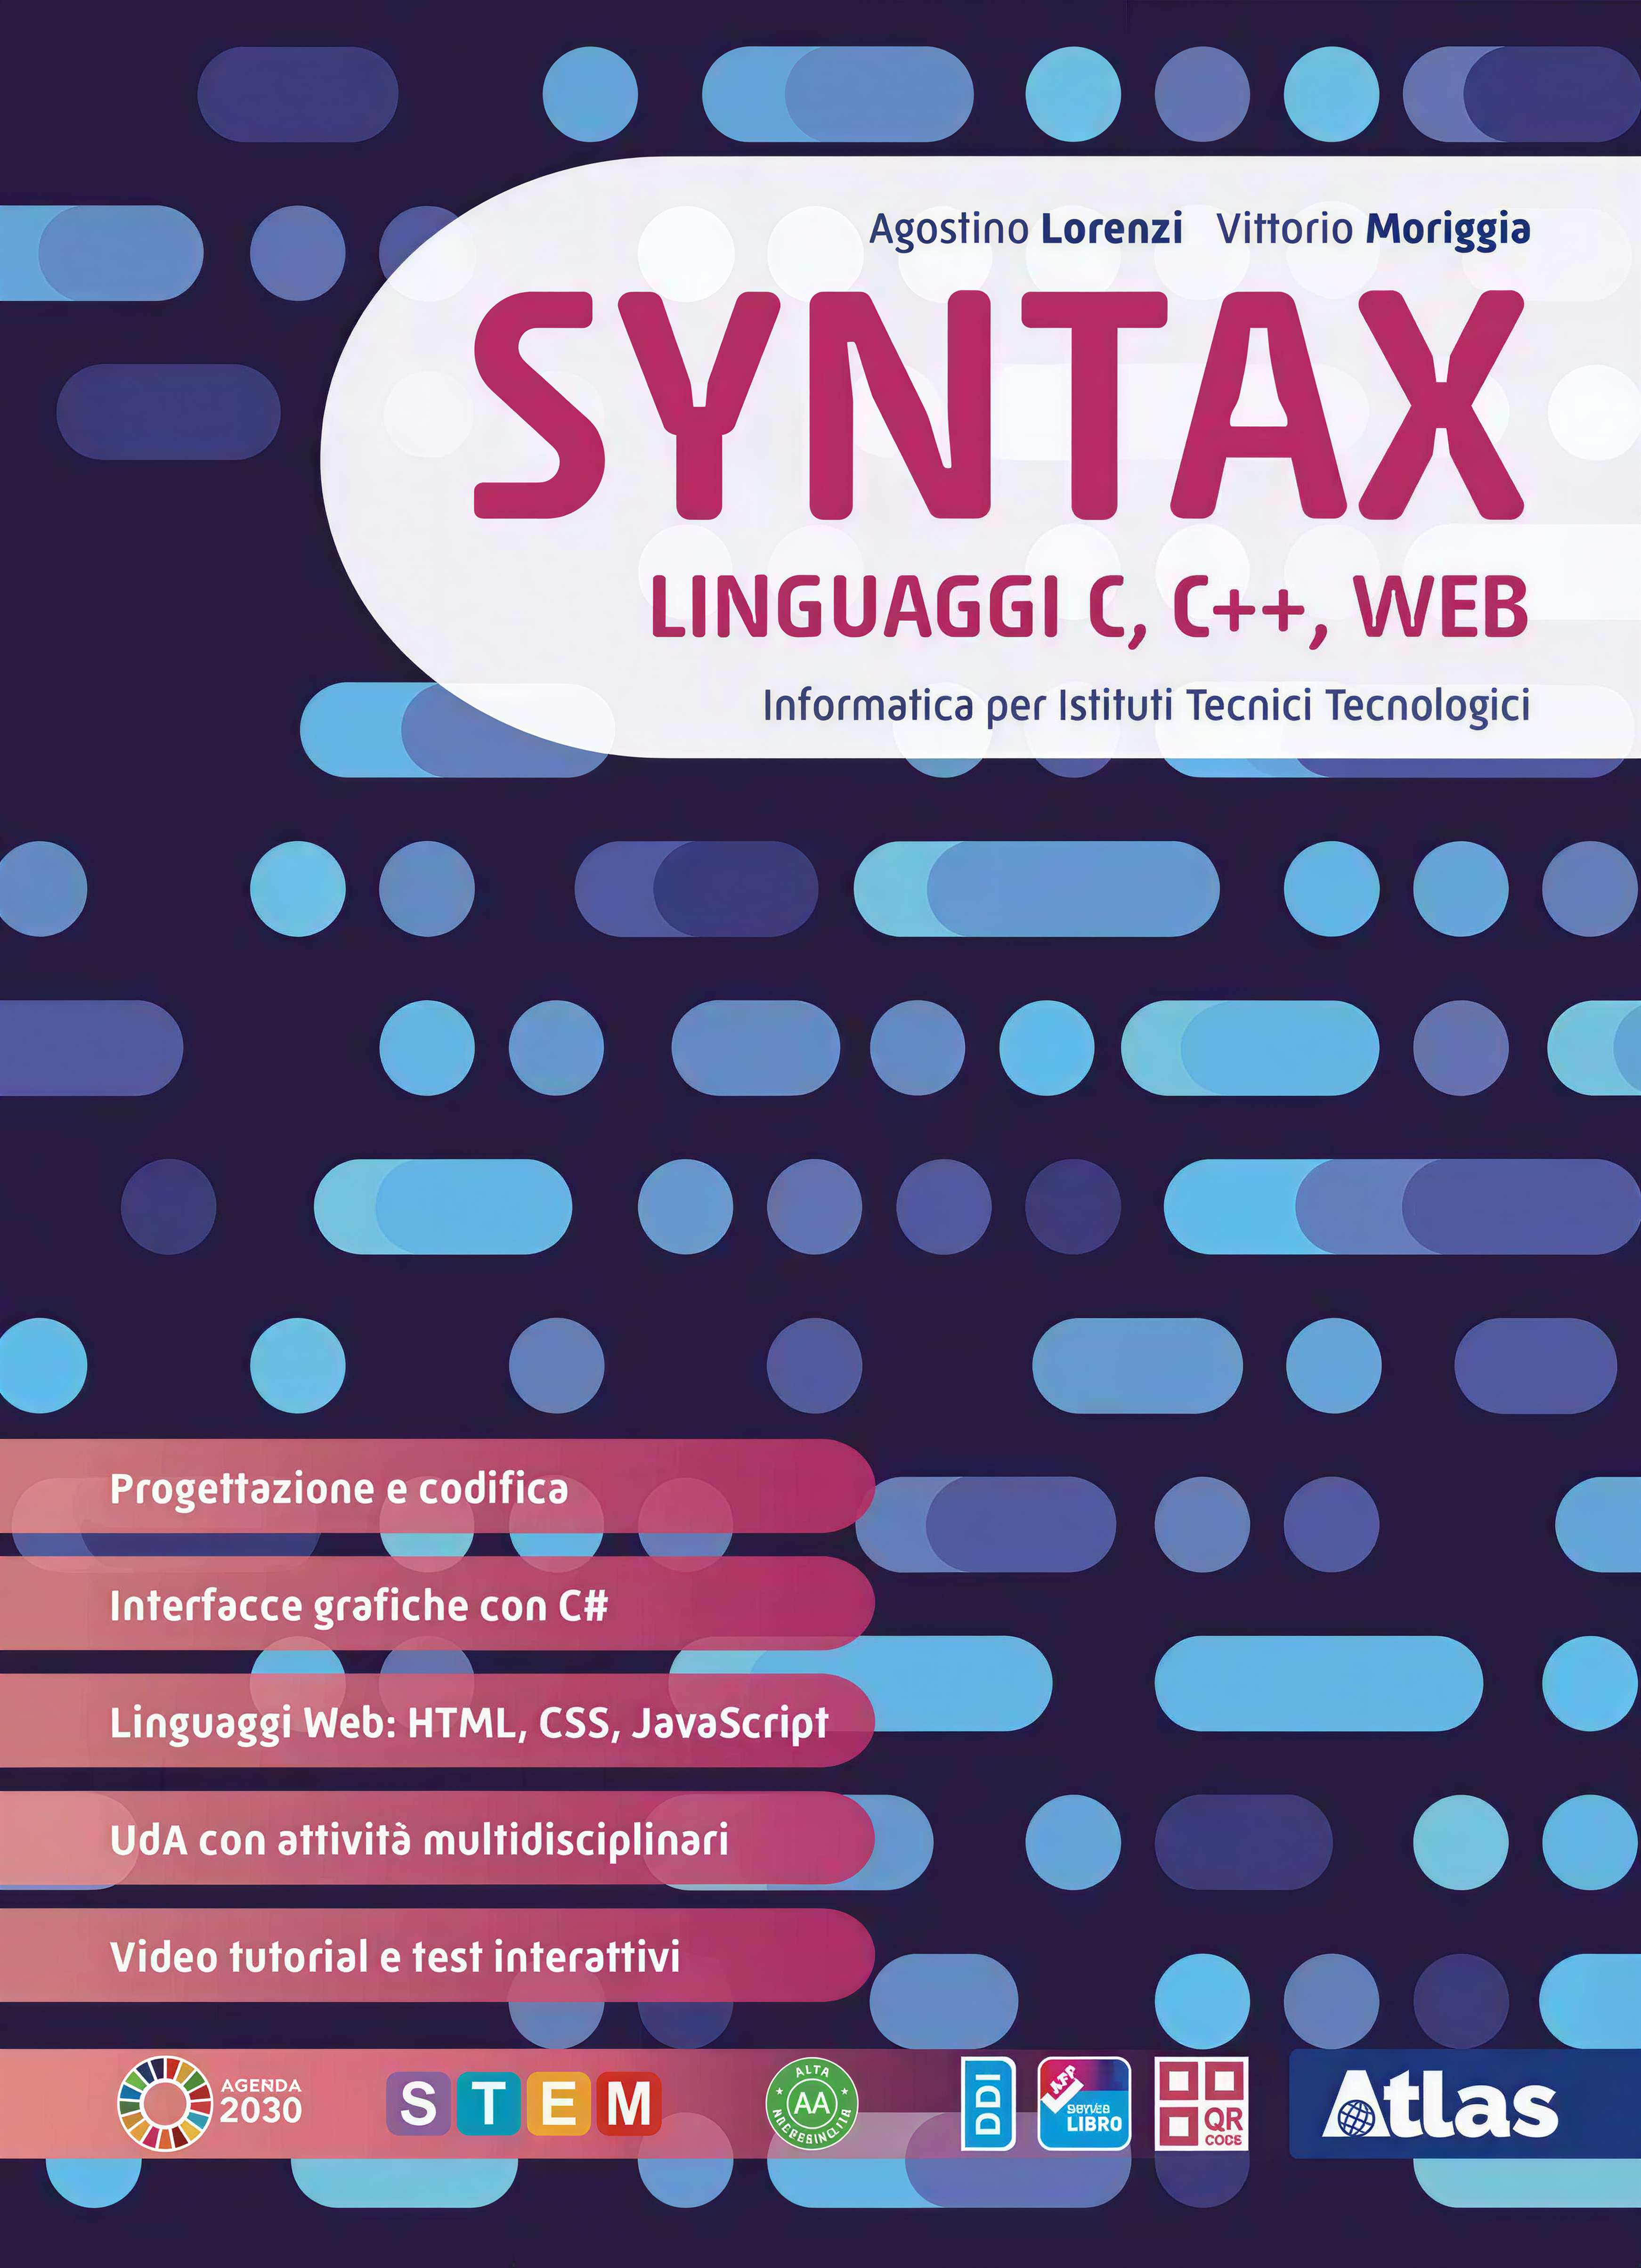
\includegraphics[width=\paperwidth]{libro.png}};
            \draw[anchor=north] (midpoint) node [fill=mainColor!30!white,fill opacity=0.9,text opacity=1,inner sep=1cm]{
                \Huge\centering\bfseries\sffamily\parbox[c][][t]{\paperwidth}
                {
                    \centering 
                    {
                        \Huge 
                        \ifsoluzioni
                            Soluzioni
                        \fi
                        Eserciziario
                    }
                    \\[15pt]
                    {\Huge TPS}
                    \\[15pt]
                    {\Large Classe III - informatica}
                    \\[20pt] 
                    {\huge Prof. Gallina Roberto}
                }
            };
        \end{tikzpicture}
    };
    \end{tikzpicture}
    \vfill
\endgroup

%----------------------------------------------------------------------------------------
%	COPYRIGHT PAGE
%----------------------------------------------------------------------------------------

\newpage
~\vfill
\thispagestyle{empty}

\noindent Copyright \copyright\ Roberto Gallina \\

\noindent Tutti i diritti riservati. \\

\noindent Questo eserciziario è stato realizzato a scopo didattico per l'uso esclusivo degli studenti dell'autore. Nessuna parte di questa opera può essere riprodotta, distribuita o trasmessa in qualsiasi forma o con qualsiasi mezzo (fotocopie, registrazioni, supporti digitali o altri) senza la previa autorizzazione scritta dell'autore, ad eccezione di brevi citazioni a scopo di recensione o critica. \\

\noindent È vietata la riproduzione per scopi commerciali o la condivisione su siti web, blog, piattaforme di condivisione di lezioni o altri spazi digitali pubblici. \\

\noindent L'autore ha curato personalmente la redazione dei contenuti. Eventuali errori, omissioni o imprecisioni sono involontari e saranno gladly corretti nelle prossime edizioni. \\

\noindent Per richieste di autorizzazione o informazioni: \\
Roberto Gallina \\
roberto.gallina@istitutoperlasca.edu.it \\


%----------------------------------------------------------------------------------------
%	TABLE OF CONTENTS
%----------------------------------------------------------------------------------------

% \chapterimage{libro.jpg}

\pagestyle{empty}

\tableofcontents

\pagestyle{fancy}

\newpage

%----------------------------------------------------------------------------------------
%	PART 1
%----------------------------------------------------------------------------------------

% \partimage{chapter_images/sistema_binario.jpg}

\part{Flowchart e pseudocodifica}

%----------------------------------------------------------------------------------------
%	CHAPTER 1
%----------------------------------------------------------------------------------------

% \chapterimage{chapter_head_1.pdf}

\chapter{Selezione e cicli}

\section{Selezione e cicli}

Risolvere i seguenti esercizi, scrivendo la pseudocodifica e il flowchart corrispondente.

\vspace{1cm}

\begin{esercizio}[1]
    Dati 4 numeri in input stampare il maggiore.
    \ifsoluzioni
        \solution

        \begin{filecontents*}{temp/fl1f.txt}
        DECLARE Integer a, b, c, d, maggiore
        INPUT Leggi a
        INPUT Leggi b
        INPUT Leggi c
        INPUT Leggi d
        PROCESS maggiore = a
        IF b > maggiore
            PROCESS maggiore = b
        END IF
        IF c > maggiore
            PROCESS maggiore = c
        END IF
        IF d > maggiore
            PROCESS maggiore = d
        END IF
        OUTPUT maggiore
        \end{filecontents*}

        \immediate\write18{python3 ../scripts/PseudocodeGenerator.py -f temp/fl1f.txt > temp/fl1p.tex}
        \input{temp/fl1p.tex}
        \newpage

        \immediate\write18{python3 ../scripts/FlowChartGenerator.py -f temp/fl1f.txt > temp/fl1f.tex}
        \input{temp/fl1f.tex}
        \newpage
    \fi
\end{esercizio}

\begin{esercizio}[1]
    Dato un numero intero N, stabilire se è pari o è dispari, ripetilo 10 volte e conta i pari e i dispari.
    \ifsoluzioni
        \solution

        ECCO LA SOLUZIONE
    \fi
\end{esercizio}

\begin{esercizio}[1]
    Date le misure dei lati di un triangolo, stabilire e il triangolo è equilatero, isoscele o scaleno.
    \ifsoluzioni
        \solution

        ECCO LA SOLUZIONE
    \fi
\end{esercizio}

\begin{esercizio}[1]
    Date le dimensioni di due rettangoli calcolarne l'area e determinare quale dei due ha superficie maggiore.
    \ifsoluzioni
        \solution

        ECCO LA SOLUZIONE
    \fi
\end{esercizio}

\begin{esercizio}[1]
    Dati 3 numeri stampare il più piccolo, il più grande e la loro media aritmetica.
    \ifsoluzioni
        \solution

        ECCO LA SOLUZIONE
    \fi
\end{esercizio}

\begin{esercizio}[2]
    Una scultura è formata da un cubo, sormontato da altri due cubi di lato rispettivamente doppio e triplo rispetto al primo cubo. Scrivere la pseudocodifica e poi il flowchart che chieda la il lato del primo cubo, assicurandosi sia valido e calcoli il volume totale della scultura e la superfice visibile totale.
    \ifsoluzioni
        \solution

        \begin{filecontents*}{temp/fl6f.txt}
        DECLARE Real l1, l2, l3
        DO
            INPUT Leggi l1
        WHILE l1 <= 0
        PROCESS l2 = 2 * l1
        PROCESS l3 = 2 * l1
        DECLARE Real s1, s2, s3
        PROCESS s1 = l1 * l1 * 6
        PROCESS s2 = l2 * l3 * 6
        PROCESS s3 = l3 * l3 * 6
        
        DECLARE Real vis
        PROCESS vis = s1 + s2 + s3
        PROCESS vis = vis - 2 * l1 - 2 * l2
        OUTPUT vis

        DECLARE Real vol
        PROCESS vol = l1 * l1 * l1 + l2 * l2 *l2 + l3 * l3 * l3
        OUTPUT vol
        \end{filecontents*}

        \immediate\write18{python3 ../scripts/PseudocodeGenerator.py -f temp/fl6f.txt > temp/fl6p.tex}
        \input{temp/fl6p.tex}
        \newpage

        \immediate\write18{python3 ../scripts/FlowChartGenerator.py -f temp/fl6f.txt > temp/fl6f.tex}
        \input{temp/fl6f.tex}
        \newpage
    \fi
\end{esercizio}

\begin{esercizio}[3]
    Una biblioteca vuole registrare il numero di libri presi in prestito durante una settimana.
    Scrivere la pseudocodifica e il flowchart che:

        richiedano in input il numero di libri prestati per ciascuno dei 7 giorni della settimana (valore non negativo);
        calcolino il numero totale di prestiti effettuati nella settimana;
        individuino il giorno con il maggior numero di prestiti;
        visualizzino il totale dei prestiti e il giorno più richiesto.
    \ifsoluzioni
        \solution

        \begin{filecontents*}{temp/fl7f.txt}
        DECLARE Integer prestiti, totale, massimo, giornoMax, giorno
        PROCESS totale = 0
        PROCESS giornoMax = 1
        FOR giorno = 1 ; giorno <= 7 ; giorno = giorno + 1
            DO
                INPUT Leggi prestiti
            WHILE prestiti < 0
            PROCESS totale = totale + prestiti
            IF giorno == 1
                PROCESS massimo = prestiti
            ELSE
                IF prestiti > massimo
                    PROCESS massimo = prestiti
                    PROCESS giornoMax = giorno
                END IF
            END IF
        END FOR
        OUTPUT totale
        OUTPUT giornoMax
        OUTPUT massimo
        \end{filecontents*}

        \immediate\write18{python3 ../scripts/PseudocodeGenerator.py -f temp/fl7f.txt > temp/fl7p.tex}
        \input{temp/fl7p.tex}
        \newpage

        \immediate\write18{python3 ../scripts/FlowChartGenerator.py -f temp/fl7f.txt > temp/fl7f.tex}
        \input{temp/fl7f.tex}
        \newpage
    \fi
\end{esercizio}

\newpage

% \immediate\write18{python3 generate/codifica_fissa_variabile.py > temp/codifica_fissa_variabile.tex}
% \input{temp/codifica_fissa_variabile.tex}

% \section{Codifiche}

% \begin{esercizio}[1]
%     \textbf{Esercizio guidato}

%     Convertire il numero 80 dalla base 10 alla base 2

%     \lipsum[1]
% \end{esercizio}


% %----------------------------------------------------------------------------------------
% %	CHAPTER 2
% %----------------------------------------------------------------------------------------

% \chapter{Sistema binario}

% \section{Conversione dalla base 10 alla base 2}

% \begin{esercizio}[1]
%     \textbf{Esercizio guidato}

%     Convertire il numero 80 dalla base 10 alla base 2

%     \lipsum[1]
% \end{esercizio}

% \section{Software}

% \begin{esercizio}[1]
%     \textbf{Esercizio guidato}

%     Convertire il numero 80 dalla base 10 alla base 2

%     \lipsum[1]
% \end{esercizio}

% %----------------------------------------------------------------------------------------
% %	CHAPTER 3
% %----------------------------------------------------------------------------------------

% % \chapterimage{chapter_head_1.pdf}

% \chapter{Codifica parole}

% \section{ASCII}

% %----------------------------------------------------------------------------------------
% %	CHAPTER 4
% %----------------------------------------------------------------------------------------

% % \chapterimage{chapter_head_1.pdf}

% \chapter{Codifica immagini}

% \section{Convertire il colore RGB in Hex}

% \section{Convertire il colore Hex in RGB}

% \section{Calcolo profondità}

% %----------------------------------------------------------------------------------------
% %	CHAPTER 5
% %----------------------------------------------------------------------------------------

% % \chapterimage{chapter_head_1.pdf}

% \chapter{Codifica suoni}

% \section{Convertire il colore RGB in Hex}

% %----------------------------------------------------------------------------------------
% %	CHAPTER 6
% %----------------------------------------------------------------------------------------

% % \chapterimage{chapter_head_1.pdf}

% \chapter{Codifica video}

% \section{Convertire il colore RGB in Hex}

%----------------------------------------------------------------------------------------
%	PART 2
%----------------------------------------------------------------------------------------

% \partimage{chapter_images/sistema_binario.jpg}

% \part{Operazioni sui dati}

%----------------------------------------------------------------------------------------
%	CHAPTER 7
%----------------------------------------------------------------------------------------

% \chapterimage{chapter_head_1.pdf}
% \chapter{Operazioni binarie}


% \section{Somma}

% Effettua le seguenti somme in binario:

% \begin{esercizio}[1]
%     \textbf{Esercizio guidato}

%     41 + 18

%     Come prima cosa convertiamo i due numeri da decimale a binario

%     % \immediate\write18{python3 ./../scripts/Dec2Bin.py 41 > temp/ex_dec2bin41.tex}
%     % \input{./temp/ex_dec2bin41.tex}

%     % \immediate\write18{python3 ./../scripts/Dec2Bin.py 18 > temp/ex_dec2bin18.tex}
%     % \input{./temp/ex_dec2bin18.tex}

%     % A questo punto eseguire la somma bit a bit, ricordando che 1+1 fa 0 con riporto di 1 e 1+1+1 fa 1 con riporto di 1

%     % \immediate\write18{python3 ./../scripts/SommaBinaria.py "41+18" > temp/ex_somma.tex}
%     % \input{./temp/ex_somma.tex}

% \end{esercizio}

% \newpage

% \begin{multicols}{2}
%     % \immediate\write18{python3 generate/somme_binarie.py > temp/somme_binarie.tex}
%     % \input{./temp/somme_binarie.tex}
% \end{multicols}

% \section{Sottrazione}

% Effettua le seguenti sottrazioni in binario:

% \begin{esercizio}[1]
%     \textbf{Esercizio guidato}

%     41 - 18

%     Come prima cosa convertiamo i due numeri da decimale a binario

%     % \immediate\write18{python3 ./../scripts/Dec2Bin.py 41 > temp/ex_dec2bin41.tex}
%     % \input{./temp/ex_dec2bin41.tex}

%     % \immediate\write18{python3 ./../scripts/Dec2Bin.py 18 > temp/ex_dec2bin18.tex}
%     % \input{./temp/ex_dec2bin18.tex}

%     % A questo punto eseguire la differenza bit a bit, ricordando che 0-1 fa 1 con il prestito di 1 dalla cifra precedente

%     % \immediate\write18{python3 ./../scripts/SottrazioneBinaria.py "41-18" > temp/ex_sottrazione.tex}
%     % \input{./temp/ex_sottrazione.tex}

% \end{esercizio}

% \newpage

% \begin{multicols}{2}
%     % \immediate\write18{python3 generate/sottrazioni_binarie.py > temp/sottrazioni_binarie.tex}
%     % \input{./temp/sottrazioni_binarie.tex}
% \end{multicols}

% \newpage

% \section{Moltiplicazione}

% Effettua le seguenti moltiplicazioni in binario:

% \begin{esercizio}[1]
%     \textbf{Esercizio guidato}

%     41 x 9

%     Come prima cosa convertiamo i due numeri da decimale a binario

%     % \immediate\write18{python3 ./../scripts/Dec2Bin.py 41 > temp/ex_dec2bin41.tex}
%     % \input{./temp/ex_dec2bin41.tex}

%     % \immediate\write18{python3 ./../scripts/Dec2Bin.py 9 > temp/ex_dec2bin9.tex}
%     % \input{./temp/ex_dec2bin9.tex}

%     % Andiamo ad eseguire la moltiplicazione del primo numero per ogni bit del secondo, ricordandosi di spostarsi di una posizione ogni volta.

%     % Al termine di deve eseguire la somma in colonna, qual'ora le righe risultimo molte conviene fare due righe per volta

%     % \immediate\write18{python3 ./../scripts/MoltiplicazioneBinaria.py "41x9" > temp/ex_moltiplicazione.tex}
%     % \input{./temp/ex_moltiplicazione.tex}

% \end{esercizio}

% \newpage

% \begin{multicols}{2}
%     % \immediate\write18{python3 generate/moltiplicazioni_binarie.py > temp/moltiplicazioni_binarie.tex}
%     % \input{./temp/moltiplicazioni_binarie.tex}
% \end{multicols}

% \newpage

% \section{Divisione}

% Effettua le seguenti divisioni in binario:

% \begin{esercizio}[1]
%     \textbf{Esercizio guidato}

%     41 : 9

%     Come prima cosa convertiamo i due numeri da decimale a binario

%     % \immediate\write18{python3 ./../scripts/Dec2Bin.py 41 > temp/ex_dec2bin41.tex}
%     % \input{./temp/ex_dec2bin41.tex}

%     % \immediate\write18{python3 ./../scripts/Dec2Bin.py 9 > temp/ex_dec2bin9.tex}
%     % \input{./temp/ex_dec2bin9.tex}

%     % Abbasso un bit alla volta fino a quando ottengo un numero maggiore o uguale del divisore, per ogni bit che abbasso mi segno uno 0 aggiunto un numero adatto mi segno un 1, scrivo il divisore sotto al numero stando attento di allineare le colonne e effettuo la sottrazione; ripeto le operazioni fino all'ultimo bit; 
    
%     % Il risultato sarà composto da quoziente e resto.

%     % \immediate\write18{python3 ./../scripts/DivisioneBinaria.py "41:9" > temp/ex_divisione.tex}
%     % \input{./temp/ex_divisione.tex}
% \end{esercizio}

% \newpage

% \begin{multicols}{2}
%     % \immediate\write18{python3 generate/divisioni_binarie.py > temp/divisioni_binarie.tex}
%     % \input{./temp/divisioni_binarie.tex}
% \end{multicols}


% %----------------------------------------------------------------------------------------
% %	CHAPTER 8
% %----------------------------------------------------------------------------------------

% % \chapter{Rilevazione e correzione errori}

% % \section{Bit di parità}

% % \section{CRC}

% % \section{LRC}

% %----------------------------------------------------------------------------------------
% %	PART 3
% %----------------------------------------------------------------------------------------

% % \partimage{chapter_images/sistema_binario.jpg}

% \part{Sistema operativo}

% %----------------------------------------------------------------------------------------
% %	CHAPTER 9
% %----------------------------------------------------------------------------------------

% % \chapterimage{chapter_head_1.pdf}
% \chapter{Scheduling}

% \section{FCFS, SJF, SRTF}

% Effettua lo schedeuling dei seguenti processi, usando l'algoritmo FCFS, SJF e SRTF:

% \begin{multicols}{2}
%     % \immediate\write18{python3 generate/sheduling1.py > temp/sheduling1.tex}
%     % \input{./temp/sheduling1.tex}
% \end{multicols}

% \newpage

% \section{Round Robin}

% Effettua lo schedeuling dei seguenti processi, usando l'algoritmo Round Robin con t=2 e t=3

% \begin{multicols}{2}
%     % \immediate\write18{python3 generate/sheduling2.py > temp/sheduling2.tex}
%     % \input{./temp/sheduling2.tex}
% \end{multicols}

% %----------------------------------------------------------------------------------------
% %	CHAPTER 10
% %----------------------------------------------------------------------------------------

% % \chapterimage{chapter_head_1.pdf}
% \chapter{Gestione memoria}

% \section{Memoria a partizione fisse}

% Mostra l'evoluzione della memoria dati i seguenti processi e la seguente memoria a partizioni fisse

% % \immediate\write18{python3 generate/allocazione_fisse.py > temp/allocazione_fisse.tex}
% % \input{./temp/allocazione_fisse.tex}

% \newpage

% \section{Memoria a partizione variabili}

% Mostra l'evoluzione della memoria dati i seguenti processi e la seguente memoria a partizioni variabili

% \immediate\write18{python3 generate/allocazione_dinamiche.py > temp/allocazione_dinamiche.tex}
% \input{./temp/allocazione_dinamiche.tex}



\end{document}